\chapter{雪盖土壤热力过程}
%\addcontentsline{toc}{chapter}{雪盖土壤热力过程}

%\begin{雪盖土壤热力过程}

在雪盖和土壤中,热力过程主要根据热传导第二定律进行描述。假设雪盖土壤无水平物质能量交换,则其垂直方向上的一维能量平衡方程如下:
\begin{equation}\label{eq:1d_energy_balance}
  c \frac{\partial T}{\partial t}=-\frac{\partial F}{\partial z}
\end{equation}
其中$c$表示雪盖或土壤的体积热容量(\unit{J.m^{-3}.K^{-1}}),$T$表示雪盖土壤温度 (K),$t$表示时间(s),$z$表示雪盖高度或土壤深度 (m),
$F$表示垂直方向的热传导通量(\unit{W.m^{-2}}),方向向上为正,表达式为$F=-\lambda\frac{\partial T}{\partial z}$,$\lambda$表示热力传导率(\unit{W.m^{-1}.K^{-1}})。
将方程(\ref{eq:1d_energy_balance})进行离散,在已知雪盖土壤表面与上边界大气交换的地表热通量$h_{\mathrm {s}} $,以及假设下边界土壤底层热通量为0的情况下,
即可求出雪盖土壤的温度廓线,之后再根据相态变化条件对温度进行进一步调整。


\section{温度求解的数值格式}\label{温度求解的数值格式}

\begin{mymdframed}{代码}
  本节对应的代码文件为\texttt{MOD\_GroundTemperature.F90}。
\end{mymdframed}

在离散上述能量平衡方程时,垂直方向上的离散方式可采用第~\ref{土壤和积雪的垂直分层} 节给出的土壤和积雪的垂直分层方案进行。
需要注意的是,在计算雪盖土壤温度之前,若有降雪发生($p_{\mathrm {snow}} >0$)且无雪盖分层($snl=0$),则此时需通过下式判断第一层雪能否形成:
\begin{equation}
  \begin{aligned}
    z_{\mathrm{sno}} &= z_{\mathrm{sno}}+\frac{p_{\mathrm{snow}} \Delta t}{\rho_{\text {sno,new }}} \\[1ex]
    W_{\mathrm{sno}} &= W_{\mathrm{sno}}+p_{\mathrm{snow}} \Delta t
  \end{aligned}
\end{equation}
其中$\rho_{\mathrm{sno,new}}$表示新降的干雪密度(\unit{kg.m^{-3}}),计算方案为~\citep{anderson1976point}:
\begin{equation}
  \rho_{\mathrm{sno, new}}=\begin{cases}
    169 & \text { 当 }\ T_{\mathrm{a}}>T_{\mathrm{frz}}+2.0 \\
    50+1.7\left(T_{\mathrm{a}}-T_{\mathrm{frz}}+15\right)^{1.5}  & \text { 当 }\ T_{\mathrm{frz}}-15.0<T_{\mathrm{a}} \leqslant T_{\mathrm{frz}}+2.0 \\
    50 & \text { 当 }\ T_{\mathrm{a}} \leqslant T_{\mathrm{frz}}-15.0
  \end{cases}
\end{equation}
若此时$z_{\mathrm{sno}} \geqslant 0.01$ \unit{m},则按第~\ref{土壤和积雪的垂直分层} 节方案对积雪进行分层,且每一层雪的温度取为$T_{\mathrm {p}} $,液态水含量取为0,固态水含量按雪层厚度权重分配$W_{\mathrm{sno}}$。若之前已有雪层且此时有降雪发生,则第一层雪的相关物理量作如下更新:
\begin{equation}
  w_{\mathrm{ice},snl+1}=w_{\mathrm{ice},snl+1}+p_{\mathrm{snow}} \Delta t
\end{equation}
\begin{equation}
  \Delta z_{snl+1}=\Delta z_{snl+1}+\frac{p_{\mathrm{snow}} \Delta t}{\rho_{\mathrm{sno, new}}}
\end{equation}
\begin{equation}
  z_{snl+1}=z_{\mathrm{h},snl+1}-0.5 \Delta z_{snl+1}
\end{equation}
\begin{equation}
  z_{\mathrm{h, snl}}=z_{\mathrm{h},snl+1}-\Delta z_{snl+1}
\end{equation}
雪盖土壤垂直分层及其热传导过程示意图见图~\ref{fig:雪盖土壤垂直分层及其热传导过程示意图}。其中土壤热力学状态变量
(如雪盖土壤温度$T_{i} $,热力传导率$\lambda_i$,体积比热容$c_i$等)定义在每一层的中间深度,从第$i+1$层到第$i$层的热传导通量$F_i$定义在两层的交界处,它可离散为:
\begin{equation}
  F_{i}=\lambda\left[z_{\mathrm{h},i}\right] \frac{T_{i}-T_{i+1}}{z_{i}-z_{i+1}}
\end{equation}
其中$\lambda\left[z_{\mathrm{h},i}\right]$表示第$i+1$层与第 $i$ 层交界处的热力传导率。求解$\lambda\left[z_{\mathrm{h},i}\right]$时,
假设从第$i+1$层到第$i$层的热传导通量等于从第$i+1$层到第$i+1$层与第$i$层交界层的热传导通量,又等于从交接层到第$i$层的热传导通量,即
\begin{equation}
  \lambda\left[z_{\mathrm{h},i}\right] \frac{T_{i}-T_{i+1}}{z_{i}-z_{i+1}}=\lambda_{i+1} \frac{T_{\mathrm{m}}-T_{i+1}}{z_{\mathrm{h},i}-z_{i+1}}=\lambda_{i} \frac{T_{i}-T_{\mathrm{m}}}{z_{i}-z_{\mathrm{h},i}}
\end{equation}
即可通过后两项解出第$i+1$层与第$i$层交界处的温度$T_{\mathrm {m}} $;再将$T_{\mathrm {m}} $代回,通过前两项即可解出$\lambda\left[z_{\mathrm{h},i}\right]$为:
\begin{equation}
  \lambda\left[z_{\mathrm{h},i}\right]=\begin{cases}
    \frac{\lambda_{i} \lambda_{i+1}\left(z_{i+1}-z_{i}\right)}{\lambda_{i}\left(z_{i+1} - z_{\mathrm{h},i}\right)+\lambda_{i+1}\left(z_{\mathrm{h},i - z_{i}}\right)} & i=snl+1, \ldots, 9 \\
    0 & i=10
  \end{cases}
\end{equation}
特殊地,对于土壤与雪盖的交界面,为防止最下层雪盖厚度过大导致$\lambda\left[z_{\mathrm{h},i}\right]$计算不准,
当$i=0$且$\left(z_{i+1}-z_{\mathrm{h},i}\right)<\left(z_{\mathrm{h},i}-z_i\right)$时,$\lambda\left[z_{\mathrm{h},i}\right]$重新计算为:
\begin{equation}
  \lambda\left[z_{\mathrm{h},i}\right]=\frac{2 \lambda_{i} \lambda_{i+1}}{\lambda_{i}+\lambda_{i+1}} \geqslant 0.5 \lambda_{i+1}
\end{equation}
{
  \begin{figure}[htbp]
    \centering
    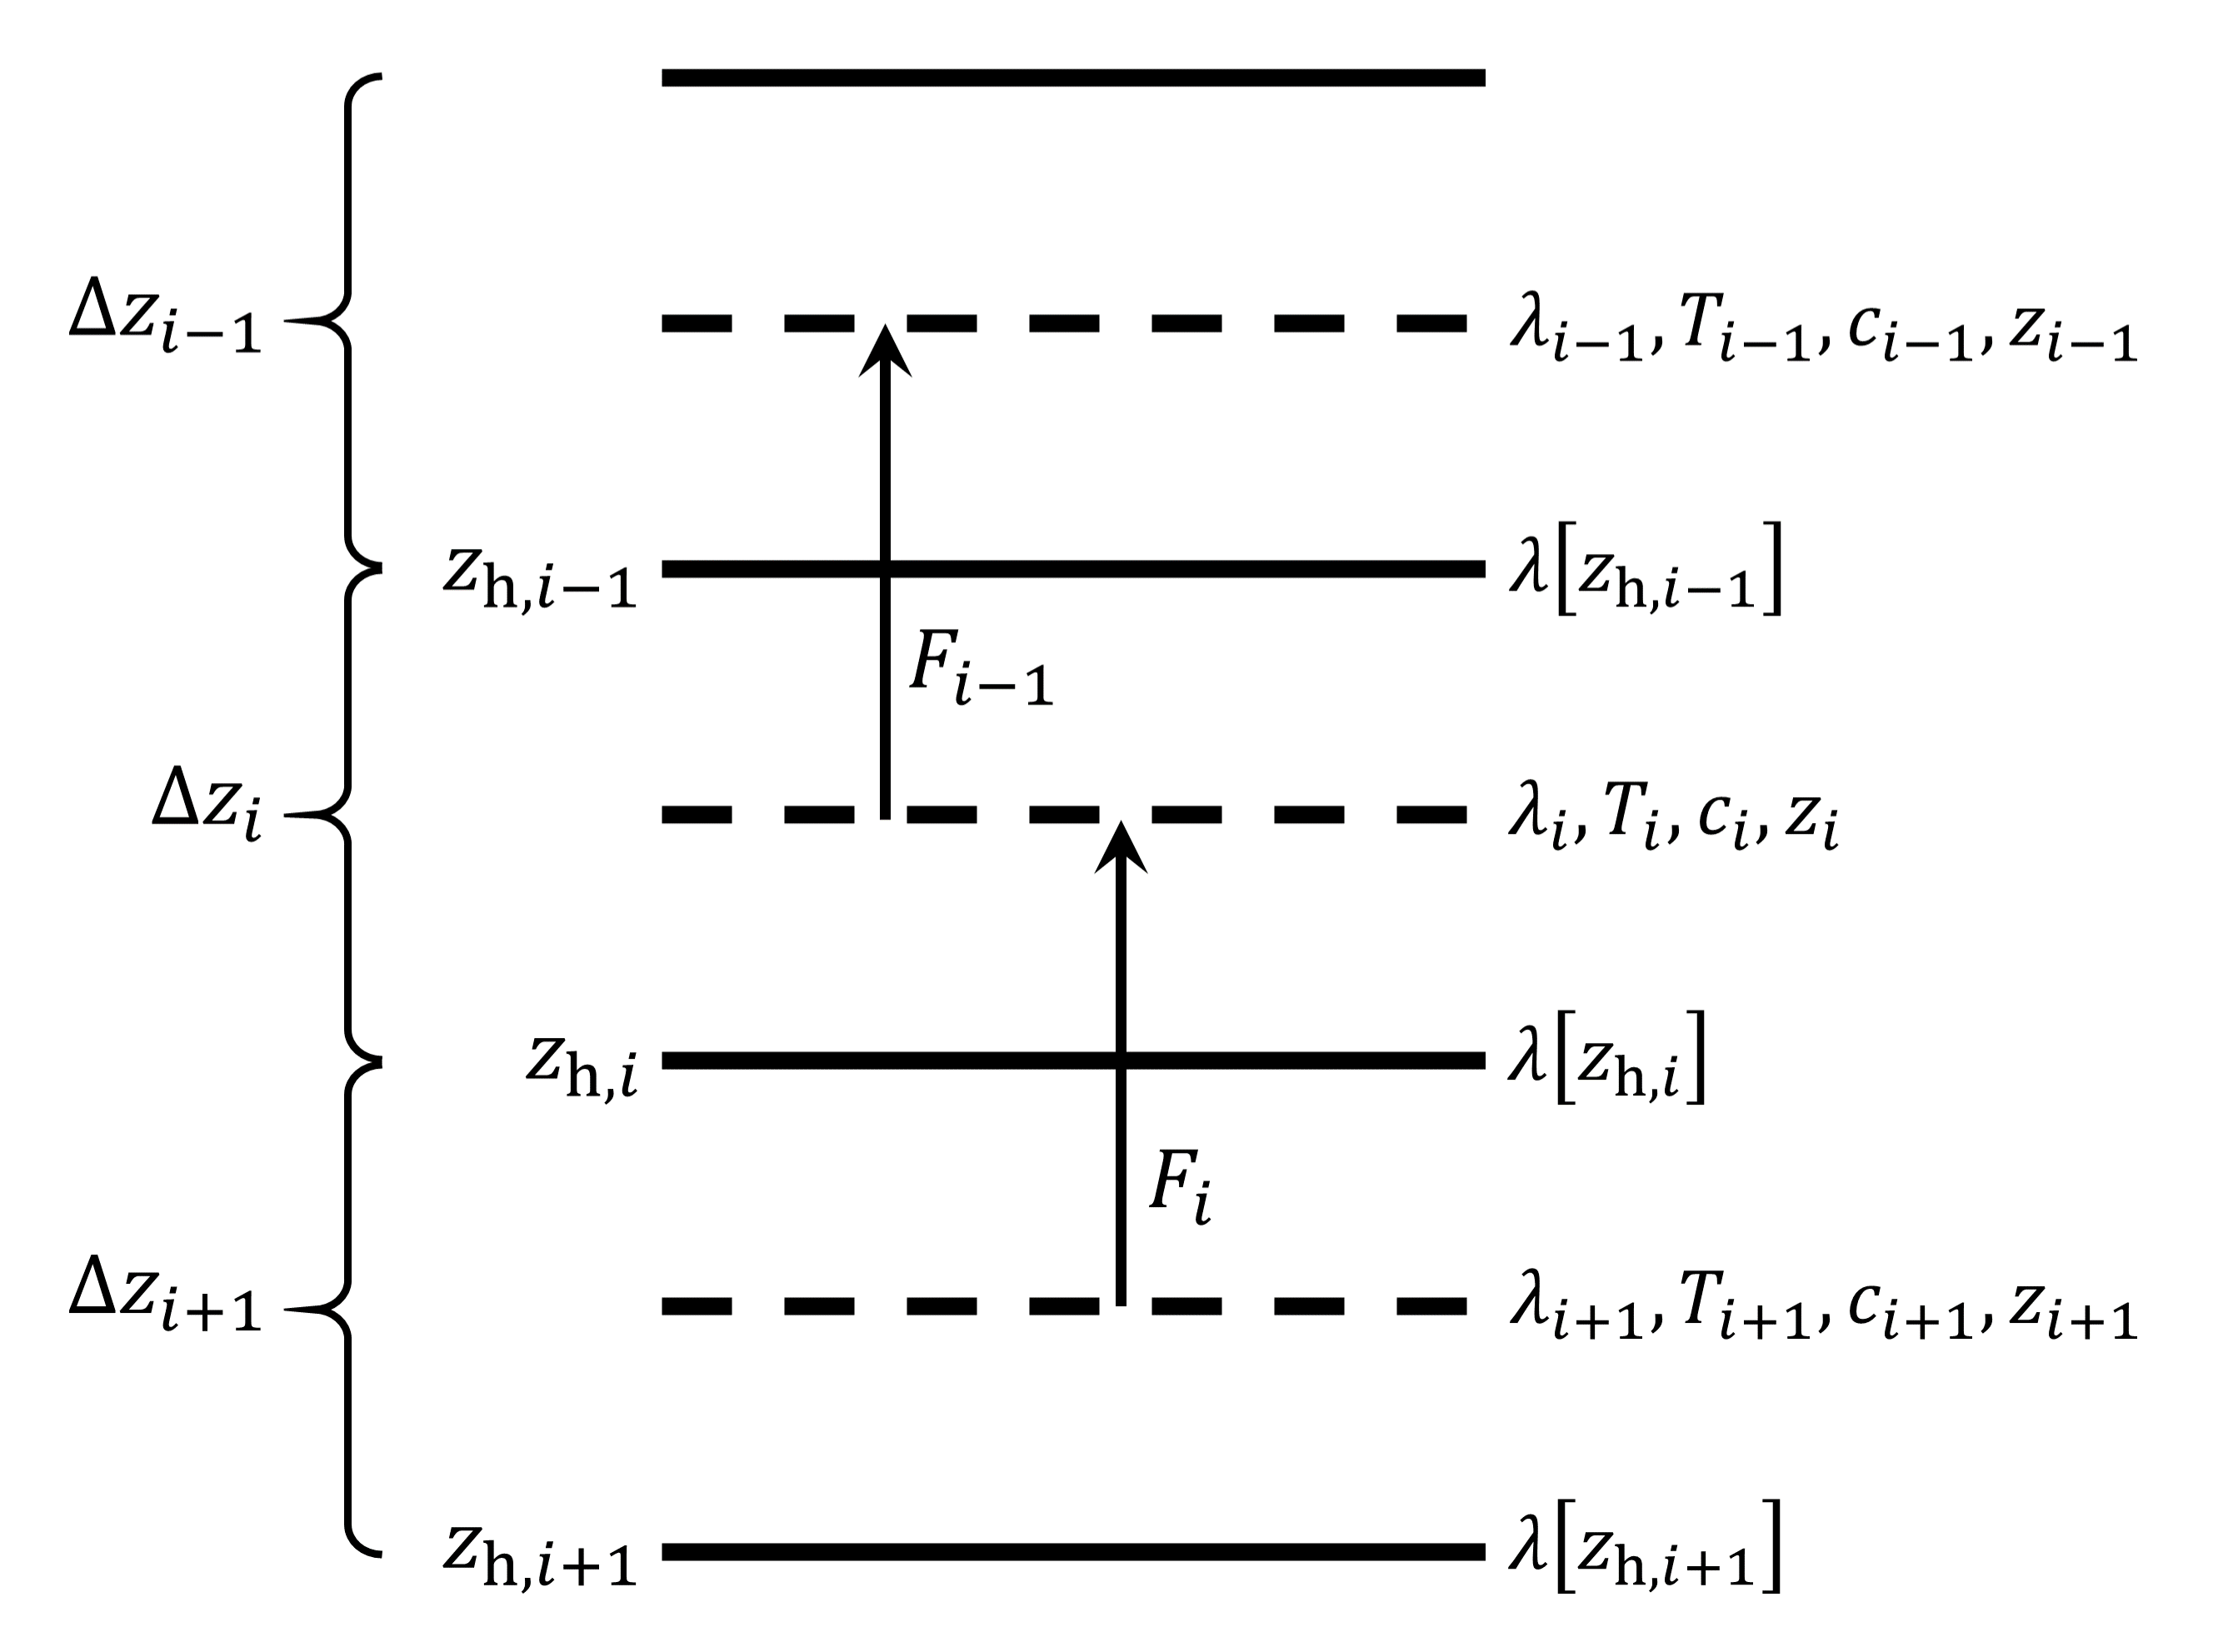
\includegraphics[width=0.7\textwidth]{Figures/雪盖土壤热力过程/雪盖土壤垂直分层及其热传导过程示意图_v2.png}
    \caption{雪盖土壤垂直分层及其热传导过程示意图}
    \label{fig:雪盖土壤垂直分层及其热传导过程示意图}
  \end{figure}
}


基于以上离散方案,第$i$层雪盖土壤的能量平衡方程可表达为:
\begin{equation}
  \frac{c_{i} \Delta z_{i}}{\Delta t}\left(T_{i}^{n+1}-T_{i}^{n}\right)=F_{i}-F_{i-1}
\end{equation}
%
其中$\Delta t$表示积分时间步长,$n$表示积分步数。此方程采用Crank--Nicholson半隐式格式求解,既包含前一时刻已有的温度与热通量信息,又包含后一时刻的预报信息。于是此方程可写为如下形式:
\begin{equation}
  \frac{c_{i} \Delta z_{i}}{\Delta t}\left(T_{i}^{n+1}-T_{i}^{n}\right)=\alpha\left(F_{i}^{n}-F_{i-1}^{n}\right)+(1-\alpha)\left(F_{i}^{n+1}-F_{i-1}^{n+1}\right)
\end{equation}
其中权重因子$\alpha=0.5$。此方程展开,即有
\begin{equation}
  \begin{aligned}
    \frac{c_{i} \Delta z_{i}}{\Delta t}\left(T_{i}^{n+1}-T_{i}^{n}\right)=& 0.5\left\{\lambda\left[z_{\mathrm{h},i}\right] \frac{T_{i}^{n}-T_{i+1}^{n}}{z_{i}-z_{i+1}}-\lambda\left[z_{\mathrm{h},i-1}\right] \frac{T_{i-1}^{n}-T_{i}^{n}}{z_{i-1}-z_{i}}\right.\\[1ex] &\left.+\lambda\left[z_{\mathrm{h},i}\right] \frac{T_{i}^{n+1}-T_{i+1}^{n+1}}{z_{i}-z_{i+1}}-\lambda\left[z_{\mathrm{h},i-1}\right] \frac{T_{i-1}^{n+1}-T_{i}^{n+1}}{z_{i-1}-z_{i}}\right\}
  \end{aligned}
\end{equation}
将所有层雪盖土壤能量平衡方程联立,可形成关于预报变量$T_{i-1}^{n+1}$,$T_i^{n+1}$和$T_{i+1}^{n+1}$的三对角方程组形式:$r_i=a_iT_{i-1}^{n+1}+b_iT_i^{n+1}+c_iT_{i+1}^{n+1}$,
其中$a_i$, $b_i$, $c_i$分别为三对角矩阵中上三角、对角线和下三角位置中的元素。用追赶法解此方程组即可快速求得每一层雪盖土壤的温度$T_i^{n+1}$。


对于雪盖土壤的中间层($snl+1<i<10$),三对角矩阵中的系数表达如下:
\begin{equation}
  \begin{aligned}
    a_{i} &= -(1-\alpha) \frac{\Delta t}{c_{i} \Delta z_{i}} \frac{\lambda\left[z_{\mathrm{h},i-1}\right]}{z_{i}-z_{i-1}} \\[1ex]
    b_{i} &= 1+(1-\alpha) \frac{\Delta t}{c_{i} \Delta z_{i}}\left[\frac{\lambda\left[z_{\mathrm{h},i-1}\right]}{z_{i}-z_{i-1}}+\frac{\lambda\left[z_{\mathrm{h},i}\right]}{z_{i+1}-z_{i}}\right] \\[1ex]
    c_{i} &= -(1-\alpha) \frac{\Delta t}{c_{i} \Delta z_{i}} \frac{\lambda\left[z_{\mathrm{h},i}\right]}{z_{i+1}-z_{i}} \\[1ex]
    r_{i} &= T_{i}^{n}+\alpha \frac{\Delta t}{c_{i} \Delta z_{i}} \lambda\left[z_{\mathrm{h},i}\right] \frac{T_{i}^{n}-T_{i+1}^{n}}{z_{i}-z_{i+1}}-\lambda\left[z_{\mathrm{h},i-1}\right] \frac{T_{i-1}^{n}-T_{i}^{n}}{z_{i-1}-z_{i}}
  \end{aligned}
\end{equation}

对于雪盖土壤的顶层和底层,需要考虑对应的边界条件:

(1) 对于雪盖土壤顶层($i=snl+1$),来自大气的热通量$h_{\mathrm {s}} $将会进入到地表中,即
\begin{equation}
  h_{\mathrm{s}}^{n+1}=-\alpha F_{i-1}^{n}-(1-\alpha) F_{i-1}^{n+1}
\end{equation}
对$h_{\mathrm {s}} ^{n+1}$采用一阶泰勒展开近似,则顶层能量平衡方程变为:
\begin{equation}
  \begin{split}
    &\mathrel{\phantom{\approx}}\frac{c_{i} \Delta z_{i}}{\Delta t}\left(T_{i}^{n+1}-T_{i}^{n}\right)=h_{\mathrm{s}}^{n+1}+\alpha F_{i}^{n}+(1-\alpha) F_{i}^{n+1} \\[1ex]
    &\approx h_{\mathrm{s}}^{n}+\frac{\partial h_{\mathrm{s}}}{\partial T_{i}}\left(T_{i}^{n+1}-T_{i}^{n}\right)+\alpha \lambda\left[z_{\mathrm{h},i}\right] \frac{T_{i}^{n}-T_{i+1}^{n}}{z_{i}-z_{i+1}}+(1-\alpha) \lambda\left[z_{\mathrm{h},i}\right] \frac{T_{i}^{n+1}-T_{i+1}^{n+1}}{z_{i}-z_{i+1}}
  \end{split}
\end{equation}
于是,基于此方程可得雪盖土壤顶层的三对角矩阵系数为:
\begin{equation}
  \begin{aligned}
    a_{i} &= 0 \\[1ex]
    b_{i} &= 1+\frac{\Delta t}{c_{i} \Delta z_{i}}\left[(1-\alpha) \frac{\lambda\left[z_{\mathrm{h},i}\right]}{z_{i+1}-z_{i}}-\frac{\partial h_{\mathrm{s}}}{\partial T_{i}}\right] \\[1ex]
    c_{i} &= -(1-\alpha) \frac{\Delta t}{c_{i} \Delta z_{i}} \frac{\lambda\left[z_{\mathrm{h},i}\right]}{z_{i+1}-z_{i}} \\[1ex]
    r_{i} &= T_{i}^{n}+\frac{\Delta t}{c_{i} \Delta z_{i}}\left[h_{\mathrm{s}}^{n}-\frac{\partial h_{\mathrm{s}}}{\partial T_{i}} T_{i}^{n}+\alpha \lambda\left[z_{\mathrm{h},i}\right] \frac{T_{i}^{n}-T_{i+1}^{n}}{z_{i}-z_{i+1}}\right]
  \end{aligned}
\end{equation}
上式将地表热通量$h_{\mathrm{s}}^n$简写为$h_{\mathrm{s}}$(\unit{W.m^{-2}})。根据地面能量平衡方程,$h_{\mathrm{s}}$计算为:
\begin{equation}
  \begin{aligned}
    h_{\mathrm{s}} &= S_{\mathrm{g}}+L_{\mathrm{g}}\left(T_{\mathrm{g}}\right)-H_{\mathrm{g}}\left(T_{\mathrm{g}}\right)-\lambda E_{\mathrm{g}}\left(T_{\mathrm{g}}\right)+H_{\mathrm{p r c g}}\left(T_{\mathrm{g}}\right) \\[1.5ex]
    \frac{\partial h_{\mathrm{s}}}{\partial T_{\mathrm{g}}} &= \frac{\partial L_{\mathrm{g}}}{\partial T_{\mathrm{g}}}-\frac{\partial H_{\mathrm{g}}}{\partial T_{\mathrm{g}}}-\frac{\partial \lambda E_{\mathrm{g}}}{\partial T_{\mathrm{g}}}+\frac{\partial H_{\mathrm{p r c g}}}{\partial T_{\mathrm{g}}}
  \end{aligned}
\end{equation}
其中$S_{\mathrm {g}} $和$L_{\mathrm {g}} $分别表示地表吸收的净太阳辐(公式~\eqref{eq:sg})和净长波辐射(公式~\eqref{eq:lg1}, \eqref{eq:lg2}) [\unit{W.m^{-2}}]。$h_{\mathrm {s}} $中感热$H_{\mathrm{g}}$和潜热$\lambda E_{\mathrm {g}} $的计算见第~\ref{ch:地表湍流通量} 章,雨水感热$H_{\mathrm{prcg}}$的计算见章节~\ref{植被地表的雨水感热}。

另外,对于潜热通量系数$\lambda$,当雪盖土壤顶层不存在液态水时,$\lambda$取为升华潜热系数$\lambda_{\mathrm {sub}} $,即:
\begin{equation}
  \lambda=\left\{\begin{array}{lr}\lambda_{\mathrm{sub}} & \text { 当 }\ w_{\mathrm{liq},snl+1}=0 \text { 并且 }\ w_{\mathrm{ice},snl+1}>0 \\ \lambda_{\mathrm{vap}} & \text { 其他情况 }\end{array}\right.
\end{equation}
其中$w_{\mathrm{liq},snl+1}$和$w_{\mathrm{ice},snl+1}$分别表示雪盖土壤顶层的液态水和固态水含量 (\unit{kg.m^{-2}},其计算见第~\ref{积雪和土壤中水分的垂直运动}~章)。

在模式中,地表温度$T_{\mathrm {g}} $与$T_{snl+1}$取为同一值,但$T_{snl+1}$表示第一层雪盖或土壤的平均温度,与实际的$T_{\mathrm {g}} $相比具有减弱的日变化幅度。 为改进这一缺陷,在求解第一层能量平衡方程时,其厚度$\Delta z_{i} $作以下调整,以求得更接近实际的$T_{\mathrm {g}}$:
\begin{equation}
\Delta z_{i}=0.5\left[z_{i}-z_{\mathrm{h},i-1}+c_{\mathrm{a}}\left(z_{i+1}-z_{\mathrm{h},i-1}\right)\right]
\end{equation}
其中调整参数$c_{\mathrm {a}} =0.34$。

(2) 对于土壤底层($i=10$),假设热传导通量为0,则能量平衡方程变为:
\begin{equation}
  \frac{c_{i} \Delta z_{i}}{\Delta t}\left(T_{i}^{n+1}-T_{i}^{n}\right)=-\alpha \lambda\left[z_{\mathrm{h},i-1}\right] \frac{T_{i-1}^{n}-T_{i}^{n}}{z_{i-1}-z_{i}}-(1-\alpha) \lambda\left[z_{\mathrm{h},i-1}\right] \frac{T_{i-1}^{n+1}-T_{i}^{n+1}}{z_{i-1}-z_{i}}
\end{equation}
于是,基于此方程可得土壤底层的三对角矩阵系数为:
\begin{equation}
  \begin{aligned}
    a_{i} &= -(1-\alpha) \frac{\Delta t}{c_{i} \Delta z_{i}} \frac{\lambda\left[z_{\mathrm{h},i-1}\right]}{z_{i}-z_{i-1}} \\
    b_{i} &= 1+(1-\alpha) \frac{\Delta t}{c_{i} \Delta z_{i}} \frac{\lambda\left[z_{\mathrm{h},i-1}\right]}{z_{i}-z_{i-1}} \\
    c_{i} &= 0 \\
    r_{i} &= T_{i}^{n}-\alpha \frac{\Delta t \lambda\left[z_{\mathrm{h},i-1}\right]}{c_{i} \Delta z_{i}} \frac{T_{i-1}^{n}-T_{i}^{n}}{z_{i-1}-z_{i}}
  \end{aligned}
\end{equation}
%
以上所涉及的各层雪盖土壤的热力传导率与体积热容量的计算方案将在~\ref{sec_thermalpar} 节给出。


\section{温度的相态变化调整}\label{sec:温度的相态变化调整}

\begin{mymdframed}{代码}
  本节对应的代码文件为\texttt{MOD\_PhaseChange.F90}。
\end{mymdframed}

通过解能量平衡方程组计算出下一时刻的雪盖土壤温度后,需要考虑相态变化过程对温度进行调整。在模式中,相态变化发生的条件为:\\
若$T_i^{n+1}>T_{\mathrm {frz}} $并且$w_{\mathrm{ice},i}>0$ \ \   \ \  \ \   固态水融化\\
若$T_i^{n+1}<T_{\mathrm {frz}} $并且$w_{\mathrm{liq},i}>0$  \ \   \ \  \ \         液态水冻结

一个特殊情况是,当土壤表面积雪存在 ($W_{\mathrm{sno}}>0$) 但并无雪层($snl=0$,$z_{\mathrm{sno}}<0.01$ \unit{m}) 时,\\
若$T_1^{n+1}>T_{\mathrm {frz}} $      \ \   \ \  \ \                 积雪融化\\
%
以上三种情况下,$T_i^{n+1}$先被调整为$T_{\mathrm {frz}} $。


相态变化的程度是由$T_{i} ^{n+1}$调整为$T_{\mathrm {frz}} $后产生的能量冗余或亏损决定的。温度调整后,能量的冗余或亏损$H_i$ (\unit{W.m^{-2}})计算如下:
\begin{equation}
  H_{i}=\begin{cases}
    h_{\mathrm{s}}^{n}+\frac{\partial h_{\mathrm{s}}}{\partial T_{i}}\left(T_{\mathrm{frz}}-T_{i}^{n}\right)+\alpha F_{i}^{n}+(1-\alpha) F_{i}^{n+1}-\frac{c_{i} \Delta z_{i}}{\Delta t}\left(T_{\mathrm{frz}}-T_{i}^{n}\right) & i=snl+1 \\
    \alpha\left(F_{i}^{n}-F_{i-1}^{n}\right)+(1-\alpha)\left(F_{i}^{n+1}-F_{i-1}^{n+1}\right)-\frac{c_{i} \Delta z_{i}}{\Delta t}\left(T_{\mathrm{frz}}-T_{i}^{n}\right) & snl+1<i<10 \\
    -\alpha F_{i-1}^{n}-(1-\alpha) F_{i-1}^{n+1}-\frac{c_{i} \Delta z_{i}}{\Delta t}\left(T_{f}-T_{i}^{n}\right) & i=10
  \end{cases}
\end{equation}
对应地,相态变化的质量调整量为$H_{\mathrm{m}}=\frac{H_{i} \Delta t}{\lambda_{\mathrm {fus}}}$,其中$\lambda_{\mathrm {fus}} $表示固态水液化潜热(\unit{J.kg^{-1}})。当固态水融化条件被满足且$H_{\mathrm {m}} >0$时,固态水含量被调整为:
\begin{equation}
  w_{\mathrm{ice},i}^{n+1}=w_{\mathrm{ice},i}^{n}-H_{\mathrm{m}} \geqslant 0
\end{equation}
当液态水冻结条件被满足且$H_{\mathrm {m}} <0$时,固态水含量被调整为:
\begin{equation}
  w_{\mathrm{ice},i}^{n+1}=\min{\left(w_{\mathrm{ice},i}^{n}-H_{\mathrm{m}}, w_{\mathrm{liq},i}^{n}+w_{\mathrm{ice},i}^{n}\right)}
\end{equation}
以上情况液态水含量均被调整为:
\begin{equation}
  w_{\mathrm{liq},i}^{n+1}=w_{\mathrm{liq},i}^{n}+w_{\mathrm{ice},i}^{n}-w_{\mathrm{ice},i}^{n+1} \geqslant 0
\end{equation}
若水分调节过程不足以消耗全部的能量冗余或填补全部的能量亏损,
则在相态变化过程之后再次进行能量结余计算:$ H_{i *}=H_{i}+\frac{\lambda_{\mathrm {fus}}\left(w_{\mathrm{ice},i}^{n+1}-w_{\mathrm{ice},i}^{n}\right)}{\Delta t}$。
若$\left|H_{i\ast}\right|>0$,则此部分能量可用来再次暖化或冷却雪盖土壤层,温度调整如下:
\begin{equation}
  T_{i}^{n+1}=\left\{\begin{array}{lr}T_{\mathrm{frz}}+\frac{\Delta t}{c_{i} \Delta z_{i}} H_{i *} /\left(1-\frac{\Delta t}{c_{i} \Delta z_{i}} \frac{\partial T_{\mathrm{s}}}{\partial T_{i}}\right) & i=s n l+1 \\ T_{\mathrm{frz}}+\frac{\Delta t}{c_{i} \Delta z_{i}} H_{i *} & i \neq s n l+1 \\ T_{\mathrm{f}} & w_{\mathrm{liq},i}^{n+1} \cdot w_{\mathrm{ice},i}^{n+1}>0\end{array}\right.
\end{equation}
对于特殊的土壤表面积雪融化的情形,当$H_{\mathrm {m}} >0$时,雪水当量减少为
\begin{equation}
  W_{\mathrm{sno}}^{n+1}=W_{\mathrm{s no}}^{n}-H_{\mathrm{m}} \geqslant 0
\end{equation}
同样,雪的厚度减少为
\begin{equation}
  z_{\mathrm{sno}}^{n+1}=\frac{W_{\mathrm{sno}}^{n+1}}{W_{\mathrm{sno}}^{n}} z_{\mathrm{sno}}^{n}
\end{equation}
若积雪融化不足以消耗全部的能量冗余,则剩余能量$H_{1\ast}$为
\begin{equation}
  H_{1 *}=H_{1}+\frac{\lambda_{\mathrm {fus}}\left(W_{\mathrm{sno}}^{n+1}-W_{\mathrm{sno}}^{n}\right)}{\Delta t}
\end{equation}
此时$H_{1\ast}$将作为新的$H_1$对第一层土壤进行上述相态变化计算。


综上,若发生土壤表面积雪融化的情形,则用于相态变化的能量累计$E$为:
\begin{equation}
  E=\frac{\lambda_{\mathrm {fus}}\left(W_{\mathrm{sno}}^{n}-W_{\mathrm{sno}}^{n+1}\right)}{\Delta t}+\sum_{i=1}^{10} \frac{\lambda_{\mathrm {fus}}\left(w_{\mathrm{ice},i}^{n}-w_{\mathrm{ice},i}^{n+1}\right)}{\Delta t}
\end{equation}
否则,
\begin{equation}
  E=\sum_{i=1}^{s n l+1} \frac{\lambda_{\mathrm {fus}}\left(w_{\mathrm{ice},i}^{n}-w_{\mathrm{ice},i}^{n+1}\right)}{\Delta t}
\end{equation}
以上过程即是雪盖土壤温度计算的全部过程。得到$T_i^{n+1}$后,地表发出的上行长波辐射$L_{\mathrm {g}} ^\uparrow$,感热通量$H_{\mathrm {g}} $与潜热通量$\lambda E_{\mathrm {g}} $需再做一次更新以作为输出的状态变量,
其中用于蒸发的水汽不能超过雪盖土壤顶层的总含水量$\left(w_{\mathrm{liq},snl+1}^{n+1}+w_{\mathrm{ice},snl+1}^{n+1}\right)/\Delta t$,
否则地表蒸发水汽取为$\left(w_{\mathrm{liq},snl+1}^{n+1}+w_{\mathrm{ice},snl+1}^{n+1}\right)/\Delta t$,产生的能量误差将加到感热通量上。


\section{雪盖土壤热力参数的计算方案}\label{sec_thermalpar}
\begin{mymdframed}{代码}
  本节对应的代码文件为\texttt{MOD\_SoilThermalParameters.F90}。
\end{mymdframed}

雪盖土壤的热力参数是完成雪盖土壤热力过程数值模拟、求解前文所述垂直方向能量平衡方程的必要输入参数,主要包含两类:雪盖土壤的体积热容量和导热率。下面就这两类参数给出在CoLM中的计算方案。

\subsection{雪盖土壤的体积热容量}

体积热容量的计算较为简单。根据 \citet{de1963thermal},土壤体积热容量由固体土壤、液态水和固态水的热容量基于各自的体积百分比加权平均得到,表达为:
\begin{equation}
  c_{i}=c_{\mathrm{s},i}\left(1-\theta_{\mathrm {sat},i}\right)+\frac{w_{\mathrm{ice},i}}{\Delta z_{i}} C_{\mathrm{ice}}+\frac{w_{\mathrm{liq},i}}{\Delta z_{i}} C_{\mathrm{liq}}
\end{equation}
其中$c_{\mathrm{s},i}$表示第$i$层的固体土壤体积热容量,由地表参数数据集提供。若地表有积雪但无雪层,则积雪的热容量也需考虑:
\begin{equation}
  c_{i}=c_{\mathrm{s},i}\left(1-\theta_{\mathrm {sat},i}\right)+\frac{w_{\mathrm{ice},i}}{\Delta z_{i}} C_{\mathrm{ice}}+\frac{w_{\mathrm{liq},i}}{\Delta z_{i}} C_{\mathrm{liq}}+\frac{W_{\mathrm{sno}}}{\Delta z_{i}} C_{\mathrm{ice}}
\end{equation}
其中,固体土壤假设由矿物质土壤、有机质土壤和砾石组成,每种成分的体积热容量基于各自的体积百分比加权平均即得到固体土壤的体积热容量。有机质土壤和砾石的体积热容量分别取值为$2.51\times 10^6$ \unit{J.m^{-3}.K^{-1}}和$2.35\times 10^6$ \unit{J.m^{-3}.K^{-1}},矿物质土壤的体积热容量(\unit{J.m^{-3}.K^{-1}})由如下方案给出:$$c_{\mathrm{minerals}}=\frac{2.128\times\%sand+2.385\times\%clay}{\%sand+\%clay}\times10^6$$
其中$\%sand$和$\%clay$表示沙土和黏土的质量百分比。

雪盖体积热容量由液态水和固态水的热容量基于各自的体积百分比加权平均得到,表达为:
\begin{equation}
  c_{i}=\frac{w_{\mathrm{ice},i}}{\Delta z_{i}} C_{\mathrm{ice}}+\frac{w_{\mathrm{liq},i}}{\Delta z_{i}} C_{\mathrm{liq}}
\end{equation}
其中,液态水和固态水的热容量可参见表~\ref{tab:物理常数}。

\subsection{雪盖土壤的导热率}

在CoLM中,土壤导热率(\unit{W.m^{-1}.K^{-1}})引入了8种计算方案供用户选择,分别为:\citet{Johansen1975}方案及其5个衍生方案(\citet{farouki1981thermal}, \citet{cote2005}, \citet{balland2005},\citet{lu2007improved}和~\citet{Yan2019thermal}),一个经验方案(\citet{tarnawski2012series})和一个理论方案(\citet{de1963thermal})。以上方案均在各自原始方案基础上,假设固体土壤由矿物质土壤、有机质土壤和砾石组成的前提下进行了改进。根据\citep{dai2019evaluation}在一定观测样本下的评估结果,\citet{balland2005}方案的模拟性能相对较优,故设为默认方案。下面将给出以上8种方案的具体计算方法。

\subsubsection{\citet{Johansen1975}方案}
\citet{Johansen1975}将土壤导热率$k$视为干土壤导热率$k_{\mathrm{dry}}$和饱和土壤导热率$k_{\mathrm{sat}}$的线性组合,其中饱和土壤导热率的权重系数为$K_{\mathrm {e}} $(称为Kersten数)。于是,土壤导热率可表达为:
\begin{equation}\label{eq:STC}
  k=(k_{\mathrm{sat}}-k_{\mathrm{dry}})K_{\mathrm {e}} +k_{\mathrm{dry}}
\end{equation}
其中,$K_{\mathrm {e}} $可视为土壤饱和度$S_{\mathrm {r}} $(定义为实际土壤含水量与饱和土壤含水量的比值)、土壤水相态和土壤粒径的函数,计算为:
\begin{equation}
  K_{\mathrm {e}} =\begin{cases}
    0.7\log_{10}S_{\mathrm {r}} +1 & \text {对于粗质颗粒的未冻结土壤且}\ S_{\mathrm {r}}>0.05\ \text {时} \\
    \log_{10}S_{\mathrm {r}} +1 & \text {对于细质颗粒的未冻结土壤且}\ S_{\mathrm {r}}>0.1\ \text {时} \\
    S_{\mathrm {r}}  & \text {对于冻结土壤时}
  \end{cases}
\end{equation}

在方程~\eqref{eq:STC} 中,干土壤导热率$k_{\mathrm{dry}}$由固体土壤各成分导热率基于其在固体土壤中的体积分数进行算术加权平均得到,计算表达式为:
\begin{equation}\label{eq:STC_dry}
  k_{\mathrm{dry}}=f_{\mathrm{minerals}}k_{\mathrm{minerals\_dry}}+f_{\mathrm{om}}k_{\mathrm{om\_dry}}+f_{\mathrm{gravel}}k_{\mathrm{gravel\_dry}}
\end{equation}
其中,$f_{\mathrm{minerals}}$,$f_{\mathrm{om}}$和$f_{\mathrm{gravel}}$分别表示矿物质土壤、有机质土壤和砾石在固体土壤中的体积分数;$k_{\mathrm{om\_dry}}$和$k_{\mathrm{gravel\_dry}}$分别表示有机质土壤和砾石在干燥状态下的整体导热率,取值为$k_{\mathrm{om\_dry}}=0.05$,$k_{\mathrm{gravel\_dry}}=0.039\theta_{\mathrm {sat}} ^{-2.2}$($\theta_{\mathrm {sat}} $表示土壤孔隙度);$k_{\mathrm{minerals\_dry}}$表示矿物质土壤在干燥状态下的导热率,计算为:$$k_{\mathrm{minerals\_dry}}=\frac{0.135\rho_{\mathrm {d}} +0.0647}{2.7-0.947\rho_{\mathrm {d}} }$$
$\rho_{\mathrm {d}} $表示矿物质土壤的干容重(\unit{g.cm^{-3}})。

饱和土壤导热率$k_{\mathrm{sat}}$由固体土壤各成分导热率和水(冰)导热率基于其体积分数进行几何加权平均得到,计算表达式为:\todo{vm和vom和vg的位置是否正确,需要检查}
\begin{equation}\label{eq:STC_wet}
  k_{\mathrm{sat}}=k_{\mathrm{minerals\_wet}}^{v_{\mathrm {m}} }k_{\mathrm{om\_wet}}^{v_{\mathrm{om}}}k_{\mathrm{gravel\_wet}}^{v_{\mathrm {g}} }k_{\mathrm {w}} ^{\theta_{\mathrm {sat}} }
\end{equation}
其中,$v_{\mathrm {m}} $,$v_{\mathrm{om}}$和$v_{\mathrm {g}} $分别表示矿物质土壤、有机质土壤和砾石在整体土壤柱内的体积分数;$k_{\mathrm{minerals\_wet}}$,$k_{\mathrm{om\_wet}}$和$k_{\mathrm{gravel\_wet}}$分别表示矿物质土壤、有机质土壤和砾石在饱和土壤状态下的整体导热率,$k_{\mathrm {w}} $表示水(冰)的导热率(参见表~\ref{tab:物理常数})。$k_{\mathrm{om\_wet}}$和$k_{\mathrm{gravel\_wet}}$分别取值为0.25和2.875;$k_{\mathrm{minerals\_wet}}$由矿物质土壤中石英部分导热率$k_{\mathrm {q}} $与非石英部分导热率$k_{\mathrm {o}} $基于其在矿物质土壤中的体积分数进行几何加权平均得到:\todo{vq和1-vq的位置是否正确,需要检查}
$$k_{\mathrm{minerals\_wet}}=k_{\mathrm {q}} ^{v_{\mathrm {q}} }k_{\mathrm {o}} ^{1-v_{\mathrm {q}} }$$
其中,$k_{\mathrm {q}} $取值为7.7,$k_{\mathrm {o}} $依据石英的体积分数$v_{\mathrm {q}} $决定:
\begin{equation}
  k_{\mathrm {o}} =\begin{cases}
    2.0 & \text {当}\ v_{\mathrm {q}} >0.2\ \text {时} \\
    3.0 & \text {当}\ v_{\mathrm {q}} \leqslant 0.2\ \text {时}
  \end{cases}
\end{equation}
$v_{\mathrm {q}} $可由~\citet{PL_98}基于12种土壤类型(依据美国农业部USDA的土壤质地分类标准)给出的经验值查表获得。

\subsubsection{\citet{farouki1981thermal}方案}
\citet{farouki1981thermal}方案作为~\citet{Johansen1975}方案的衍生方案,土壤导热率$k$与干土壤导热率$k_{\mathrm{dry}}$的计算方式完全一致(\eqref{eq:STC} 和~\eqref{eq:STC_dry})。饱和土壤导热率$k_{\mathrm{sat}}$由固体土壤导热率和水(冰)导热率基于其体积分数进行几何加权平均得到,而固体土壤导热率取值为各成分导热率基于其在固体土壤中的体积分数的算术加权平均值。$k_{\mathrm{sat}}$计算表达式为:\todo{$\theta_{sat}$的位置是否正确,需要检查}
\begin{equation}\label{eq:STC_wet_Farouki}
  k_{\mathrm{sat}}=(f_{\mathrm{minerals}}k_{\mathrm{minerals\_wet}}+f_{\mathrm{om}}k_{\mathrm{om\_wet}}+f_{\mathrm{gravel}}k_{\mathrm{gravel\_wet}})^{1-\theta_{\mathrm {sat}} }k_{\mathrm {w}} ^{\theta_{\mathrm {sat}} }
\end{equation}
其中,$k_{\mathrm{minerals\_wet}}$也与~\citet{Johansen1975}方案的计算方式不同,表达为:$$k_{\mathrm{minerals\_wet}}=\frac{8.80\times\%sand+2.92\times\%clay}{\%sand+\%clay}$$
其中$\%sand$和$\%clay$表示沙土和黏土的质量百分比。

Kersten数$K_{\mathrm {e}} $的计算方式相较~\citet{Johansen1975}方案更为简化,表达为:
\begin{equation}
  K_{\mathrm {e}} =\begin{cases}
    \log_{10}S_{\mathrm {r}} +1 & \text {对于未冻结土壤时} \\
    S_{\mathrm {r}}  & \text {对于冻结土壤时}
  \end{cases}
\end{equation}

\subsubsection{\citet{cote2005}方案}
在~\citet{cote2005}方案中,土壤导热率$k$与饱和土壤导热率$k_{\mathrm{sat}}$的计算方式与~\citet{Johansen1975}方案完全一致 (\eqref{eq:STC} 和~\eqref{eq:STC_wet})。而干土壤导热率$k_{\mathrm{dry}}$和Kersten数$K_{\mathrm {e}} $的计算方案则通过大量实测数据拟合得到经验关系式。$k_{\mathrm{dry}}$表达为:
\begin{equation}\label{eq:STC_dry_CK}
  k_{\mathrm{dry}}=\sum_if_{i} \chi_{i} (10^{-\eta_i\theta_{\mathrm {sat}} }),\quad i=\text{矿物质土壤、有机质土壤或砾石}
\end{equation}
$K_{\mathrm {e}} $表达为:
\begin{equation}
  K_{\mathrm {e}} =\frac{\kappa S_{\mathrm {r}} }{1+(\kappa -1)S_{\mathrm {r}} }
\end{equation}
其中$\chi_i$、$\eta_i$和$\kappa$为经验参数,按照表~\ref{tab:Cote2005方案中k计算参数取值} 和~\ref{tab:Cote2005方案中k计算参数kappa取值} 取值:
\begin{table}[htbp]
  \centering
  \caption{\citet{cote2005}方案中$k_{\mathrm{dry}}$计算公式中的参数取值}
  \label{tab:Cote2005方案中k计算参数取值}
  \begin{tabular}{@{}lcc@{}}
    \toprule
    土壤成分   & $\chi$       & $\eta$             \\
    \midrule
    砾石       & 1.70         & 1.80               \\
    有机质土壤 & 0.30         & 0.87               \\
    矿物质土壤 & 0.75         & 1.20               \\
    \bottomrule
  \end{tabular}
\end{table}
%
\begin{table}[htbp]
  \centering
  \caption{\citet{cote2005}方案中$K_{\mathrm {e}} $计算公式中$\kappa$的参数取值}
  \label{tab:Cote2005方案中k计算参数kappa取值}
  \begin{tabular}{@{}lcccc@{}}
    \toprule
    土壤状态   & 粗质颗粒土壤 & 中等颗粒或砂质土壤  & 粉粒或黏粒土壤 & 有机质土壤 \\
    \midrule
    未冻结土壤 & 4.60         & 3.55                & 1.90           & 0.60       \\
    冻结土壤   & 1.70         & 0.95                & 0.85           & 0.25       \\
    \bottomrule
  \end{tabular}
\end{table}

\subsubsection{\citet{balland2005}方案}
在~\citet{balland2005}方案中,土壤导热率$k$、干土壤导热率$k_{\mathrm{dry}}$和饱和土壤导热率$k_{\mathrm{sat}}$的计算方式与~\citet{Johansen1975}方案完全一致 (\eqref{eq:STC},\eqref{eq:STC_dry} 和~\eqref{eq:STC_wet})。而Kersten数$K_{\mathrm {e}} $的计算方案则通过大量实测数据得到从干土壤到饱和土壤、细颗粒土壤到粗颗粒土壤过渡更为平滑的计算方式,表达式为:
\begin{equation}
  K_{\mathrm {e}} =\begin{cases}
    S_{\mathrm {r}} ^{0.5(1+v_{\mathrm{om}}-\alpha v_{\mathrm{sand}}-v_{\mathrm {g}} )}\left[\left(\frac{1}{1+{\mathrm e}^{-\beta S_{\mathrm {r}} }}\right)^3-\left(\frac{1-S_{\mathrm {r}} }{2}\right)^3\right]^{1-v_{\mathrm{om}}} & \text {对于未冻结土壤时} \\
    S_{\mathrm {r}} ^{1+v_{\mathrm{om}}} & \text {对于冻结土壤时}
  \end{cases}
\end{equation}
其中,$v_{\mathrm{sand}}$、$v_{\mathrm{om}}$和$v_{\mathrm {g}} $分别表示砂质土壤、有机质土壤和砾石在整体土壤柱内的体积分数。$\alpha$和$\beta$为经验参数,取值见表~\ref{tab:Balland-Arp方案中Ke计算参数取值} (来自~\citet{Barry2015thermal})。

{
  \begin{table}[htbp]
    \centering
    \caption{\citet{balland2005}方案中$K_{\mathrm {e}} $计算公式中的参数取值}
    \label{tab:Balland-Arp方案中Ke计算参数取值}
    \begin{tabular}{@{}lcc@{}}
      \toprule
      土壤成分     & $\alpha$ & $\beta$ \\
      \midrule
      粗质颗粒土壤 & 0.38     & 35.0    \\
      中等颗粒土壤 & 0.24     & 26.0    \\
      细质颗粒土壤 & 0.20     & 10.0    \\
      \bottomrule
    \end{tabular}
  \end{table}
}


\subsubsection{\citet{lu2007improved}方案}
在~\citet{lu2007improved}方案中,土壤导热率$k$与饱和土壤导热率$k_{\mathrm{sat}}$的计算方式与~\citet{Johansen1975}方案完全一致(\eqref{eq:STC} 和~\eqref{eq:STC_wet})。而干土壤导热率$k_{\mathrm{dry}}$也沿用~\citet{Johansen1975}方案中的计算公式~\eqref{eq:STC_dry},但矿物质土壤在干燥状态下的导热率$k_{\mathrm{minerals\_dry}}$则通过观测数据重新拟合了新的公式,表达为:
\begin{equation}\label{eq:STC_dry_Lu}
  k_{\mathrm{minerals\_dry}}=-0.56\theta_{\mathrm {sat}} +0.51
\end{equation}

此外,Kersten数$K_{\mathrm {e}} $的计算方案也通过大量实测数据拟合得到了新的经验关系式,表达为:
$$K_{\mathrm {e}} ={\mathrm e}^{\alpha\left(1-S_{\mathrm {r}} ^{\alpha-\beta}\right)}$$
其中,$\alpha$和$\beta$为经验参数,取值见表~\ref{tab:lu2007方案中Ke参数取值}。

{
  \begin{table}[htbp]
    \centering
    \caption{\citet{lu2007improved}方案中$K_{\mathrm {e}} $计算公式中的参数取值}
    \label{tab:lu2007方案中Ke参数取值}
    \begin{tabular}{@{}lcc@{}}
      \toprule
      土壤成分     & $\alpha$ & $\beta$ \\
      \midrule
      粗质颗粒土壤 & 0.728    & 1.165   \\
      细质颗粒土壤 & 0.37     & 1.29    \\
      \bottomrule
    \end{tabular}
  \end{table}
}


\subsubsection{\citet{Yan2019thermal}方案}
在~\citet{Yan2019thermal}方案中,土壤导热率$k$与饱和土壤导热率$k_{\mathrm{sat}}$的计算方式与~\citet{Johansen1975}方案完全一致 (\eqref{eq:STC} 和~\eqref{eq:STC_wet})。而干土壤导热率$k_{\mathrm{dry}}$则通过观测数据重新拟合了新的公式,表达为:
\begin{equation}\label{eq:STC_dry_Yan}
  k_{\mathrm{dry}}=-0.5815\theta_{\mathrm {sat}}  + 0.4999
\end{equation}

此外,Kersten数$K_{\mathrm {e}} $的计算方案也通过大量实测数据拟合得到了新的经验关系式,表达为:$$K_{\mathrm {e}} =\frac{1+\left(\frac{\theta_{\mathrm {sat}} }{\beta}\right)^{-\beta}}{1+\left(\frac{\theta_{\mathrm{liq}}}{\beta}\right)^{-\beta}}$$
其中,$\theta_{\mathrm{liq}}$表示液态土壤体积含水量,$\beta$为经验参数,表达为:$$\beta = -0.303k_{\mathrm{sat}} - 0.201m_{\mathrm{sand}} + 1.532$$
$m_{\mathrm{sand}}$表示砂质土壤在整体土壤柱内的质量分数。

\subsubsection{\citet{tarnawski2012series}方案}
在~\citet{Johansen1975}方案及其衍生方案中,假设土壤组分的排列方式在热流方向上是并行的或处在并行和串行之间的某种方式,因此总热导率可计算为所有土壤组分热导率的算术或几何平均值。作为更为复杂的方案,\citet{tarnawski2012series}提出了一种基于土壤组分串行-并行混合排列下的土壤导热率计算方案。他们假设热流通过三种介质通道传导,即固体均匀介质通道($\Theta_{\mathrm{sb}}$),由土壤固体与一部分土壤水($n_{\mathrm {w}} $)和一部分土壤空气($n_{\mathrm {a}} $)的并联路径相连构成的串行-并行通道,以及土壤水($\Theta_{\mathrm {w}} $)和空气($\Theta_{\mathrm {a}} $)并行排列的通道。括号中的符号表示土壤中每个组分的体积分数。通过将经典电阻模型应用于每个热流通道,\citet{tarnawski2012series}提出的总热导率计算方案可以通过以下方程计算:
\begin{equation}
  \begin{aligned}
    k=&k_{\mathrm {s}} \Theta_{\mathrm{sb}}+\frac{(1-\theta_{\mathrm {sat}} -\Theta_{\mathrm{sb}}+n_{\mathrm{wm}})^2}{\frac{1-\theta_{\mathrm {sat}} -\Theta_{\mathrm{sb}}}{k_{\mathrm {s}} }+\frac{n_{\mathrm{wm}}}{k_{\mathrm {w}} \frac{n_{\mathrm {w}} }{n_{\mathrm{wm}}}+k_{\mathrm {a}} \left(1-\frac{n_{\mathrm {w}} }{n_{\mathrm{wm}}}\right)}}+k_{\mathrm {w}} \left(\theta_{\mathrm {sat}}S_{\mathrm {r}} -n_{\mathrm{wm}}\frac{n_{\mathrm {w}} }{n_{\mathrm{wm}}}\right) \\
    +&k_{\mathrm {a}} \left[\theta_{\mathrm {sat}} (1-S_{\mathrm {r}} )-n_{\mathrm{wm}}\left(1-\frac{n_{\mathrm {w}} }{n_{\mathrm{wm}}}\right)\right]
  \end{aligned}
\end{equation}
其中,$k_{\mathrm {s}} $,$k_{\mathrm {w}} $和$k_{\mathrm {a}} $分别表示固体土壤、水(冰)和空气的导热率,而固体土壤导热率由矿物质土壤、有机质土壤和砾石在饱和土壤状态下的导热率基于其体积分数进行几何加权平均得到,每种土壤组分在饱和状态下的导热率计算方案与~\citet{Johansen1975}方案完全一致。$\Theta_{\mathrm{sb}}$和$n_{\mathrm{wm}}$可通过砾石和砂质土壤含量拟合得到,计算表达式为:$$\Theta_{\mathrm{sb}}=0.0237-0.0175\left(m_{\mathrm{gravel}}+m_{\mathrm{sand}}\right)^3$$$$n_{\mathrm{wm}}=n_{\mathrm {a}} +n_{\mathrm {w}} =0.088-0.037\left(m_{\mathrm{gravel}}+m_{\mathrm{sand}}\right)^3$$
其中,$m_{\mathrm{gravel}}$和$m_{\mathrm{sand}}$表示砾石和砂质土壤在整体土壤柱内的质量分数。$\frac{n_{\mathrm {w}} }{n_{\mathrm{wm}}}$可由如下关系近似得到:
\begin{equation}
  \frac{n_{\mathrm {w}} }{n_{\mathrm{wm}}}=\begin{cases}
    0  & \text{当}\ Sr=0\ \text{时} \\
    {\mathrm e}^{1-S_{\mathrm {r}} ^{-X}} & \text{当}\ 0<S_{\mathrm {r}} \leqslant1 \text{时}
  \end{cases}
\end{equation}
其中,$X=0.6-0.3\left(m_{\mathrm{gravel}}+m_{\mathrm{sand}}\right)^3$为表征小土壤空隙持水能力的因子。

\subsubsection{\citet{de1963thermal}方案}
\citet{de1963thermal}方案是一种经典的理论方案,其发展基于麦克斯韦方程。在该方案中,假设土壤结构由椭球形颗粒组成,这些颗粒在连续的孔隙流体(空气或水)中可自由浮动。因此,土壤总热导率可被估算为考虑土壤各组分形状因子的基础上各热导率的加权平均值,表达式如下:$$k=\frac{F_{\mathrm {w}} \theta_{\mathrm {sat}}S_{\mathrm {r}}k_{\mathrm {w}} +F_{\mathrm {a}} \theta_{\mathrm {sat}} \left(1-S_{\mathrm {r}} \right)k_{\mathrm {a}} +F_{\mathrm {s}} \left(1-\theta_{\mathrm {sat}} \right)k_{\mathrm {s}} }{F_{\mathrm {w}} \theta_{\mathrm {sat}}S_{\mathrm {r}} +F_{\mathrm {a}} \theta_{\mathrm {sat}} \left(1-S_{\mathrm {r}} \right)+F_{\mathrm {s}} \left(1-\theta_{\mathrm {sat}} \right)}$$
其中,$F_{\mathrm {s}} $、$F_{\mathrm {w}} $和$F_{\mathrm {a}} $分别表示固体土壤、水和空气的形状因子,它们可通过如下经验公式得到:
\begin{equation}
  F_{i} =\frac{1}{3}\left[\frac{2}{1+\left(\frac{k_{i} }{k_{\mathrm {w}} }-1\right)g_{i} }+\frac{1}{1+\left(\frac{k_{i} }{k_{\mathrm {w}} }-1\right)(1-2g_{i} )}\right],\quad i=w,a,s
\end{equation}
$g_{i} $为表征椭球形颗粒的拟合参数,可由下式计算:
\begin{equation}
  g_{i} =\begin{cases}
    0.013+0.944\theta_{\mathrm {sat}}S_{\mathrm {r}}   & \text{对于空气分子且}\ \theta_{\mathrm {sat}}S_{\mathrm {r}} \leqslant 0.09\ \text{时} \\
    0.333-\left(0.333-0.035\right)\left(1-S_{\mathrm {r}} \right) & \text{对于空气分子且}\ \theta_{\mathrm {sat}}S_{\mathrm {r}} >0.09\ \text{时} \\
    0.125 &\text{对于固体土壤颗粒}
  \end{cases}
\end{equation}


\subsubsection{积雪导热率计算方案}
根据~\citet{jordan1991one},雪盖热力传导率$\lambda_{i} $ (\unit{W.m^{-1}.K^{-1}}, $i=snl+1,\ldots,0$)的计算公式如下:
\begin{equation}
  \lambda_{i}=k_{\mathrm {a}}+\left(7.75 \times 10^{-5} \rho_{\mathrm{sno},i}+1.105 \times 10^{-6} \rho_{\mathrm{sno},i}^{2}\right)\left(k_{\mathrm {ice}}-k_{\mathrm {a}}\right)
\end{equation}
其中$k_{\mathrm {a}} $表示空气的热力传导率(\unit{W.m^{-1}.K^{-1}}),$\rho_{\mathrm{sno},i}$表示第 $i$ 层雪的平均密度(\unit{kg.m^{-3}}):
\begin{equation}
  \rho_{\mathrm{sno},i}=\frac{w_{\mathrm{liq},i}+w_{\mathrm{ice},i}}{\Delta z_{i}}
\end{equation}
